\section{Motivation for Tool Support}

Research artifacts in software engineering become more valuable when they can be
used in realistic workflows. A model that classifies minimap images in an
offline experiment demonstrates feasibility, but developers work inside IDEs,
version-control systems, code-review platforms, and continuous-integration
pipelines. Therefore, one of the objectives of this doctoral project is to
connect minimap-based analysis to practical development environments.

The tool-support line is named \textit{MinimapSignatures}. Its purpose is to
operationalize source code minimaps as visual signatures inside IDEs. The tool
does not replace syntax highlighting, code navigation, static-analysis warnings,
or dependency inspection. Instead, it adds a model-based visual-analysis layer:
the active source file is transformed into an anonymized minimap, sent to a
backend, classified by trained models, and returned to the IDE as developer-facing
feedback.

This tool line contributes to the thesis in three ways. First, it validates that
minimap generation can be executed locally in development environments. Second,
it shows that the same backend contract can support different IDE clients.
Third, it creates infrastructure for future evaluations involving multi-file
analysis, project-specific models, code quality indicators, and developer
feedback.

\section{Architecture}

MinimapSignatures follows a client--server architecture. The clients are IDE
plugins for Visual Studio Code and IntelliJ IDEA. The server is a Python backend
responsible for receiving minimap images, preprocessing them, invoking trained
models, and returning structured predictions. Figure~\ref{fig:tool-architecture}
illustrates the architecture.

\begin{figure}[ht]
    \centering
    \caption{Architecture of the MinimapSignatures ecosystem.}
    \label{fig:tool-architecture}
    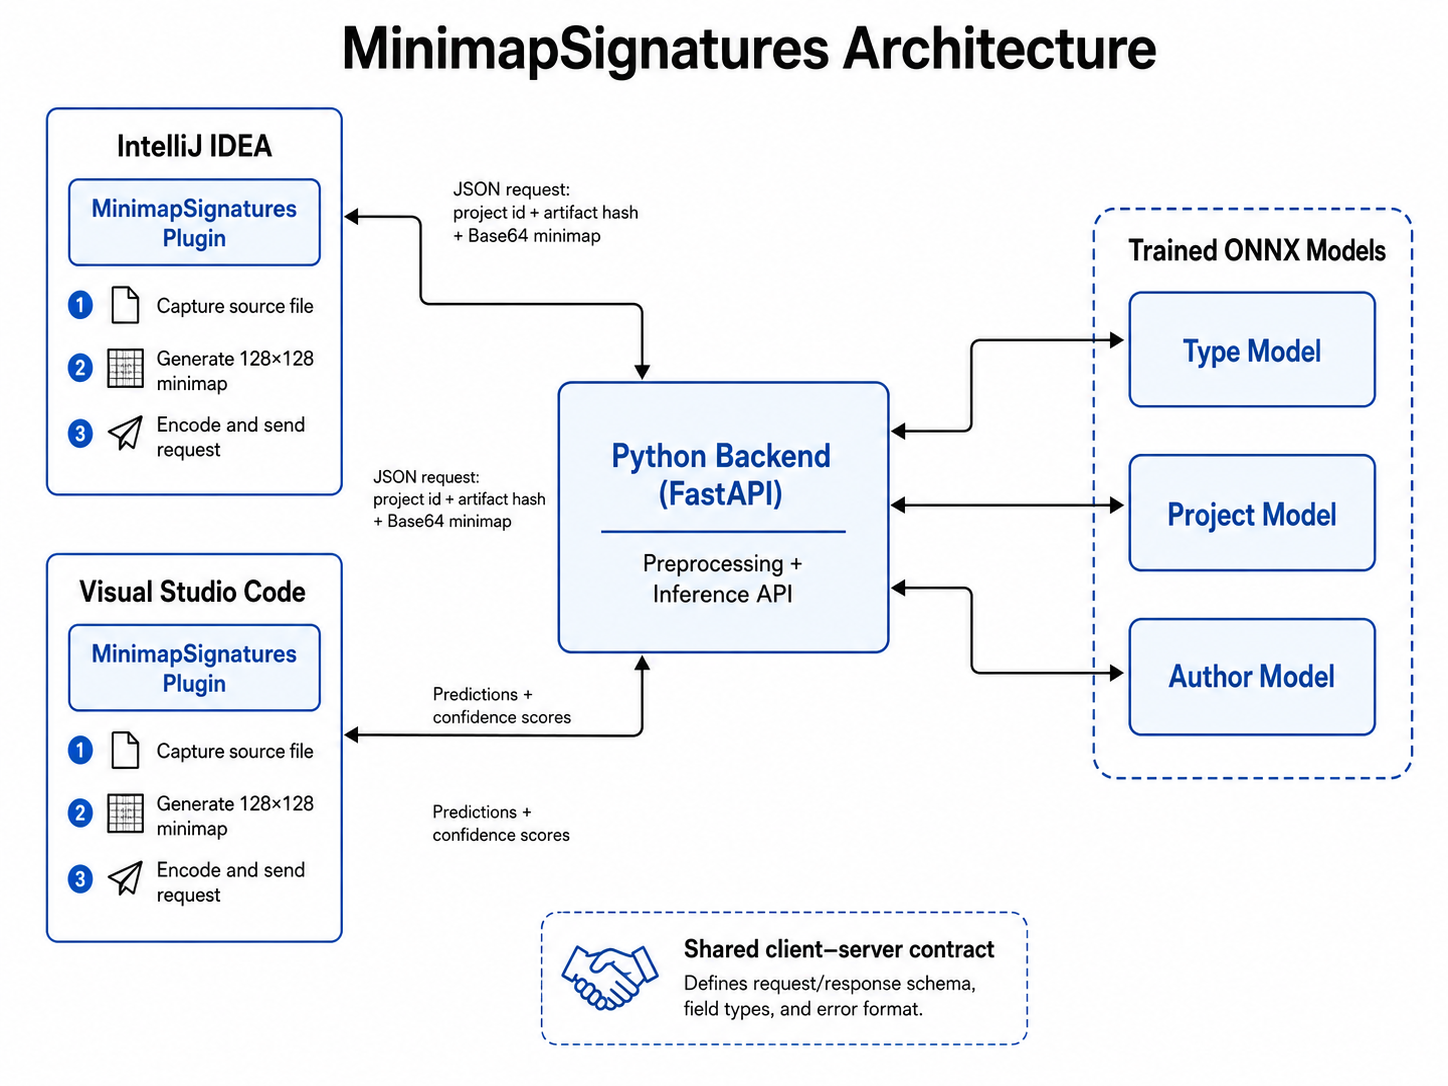
\includegraphics[width=0.92\textwidth]{figuras/minimapsignatures-architecture.png}
    \fautor
\end{figure}

The separation between clients and backend is a central design decision. IDE
plugins should remain lightweight because each IDE has its own APIs, packaging
requirements, and interaction patterns. Model inference, on the other hand, may
change frequently as new architectures, datasets, and objectives are introduced.
By decoupling them, the project can update the backend without rewriting each
plugin.

\section{Backend Service}

The backend is implemented in Python and exposes an HTTP interface. Its main
endpoint receives a JSON payload containing metadata and a base64-encoded PNG
image representing the minimap. The backend decodes the image, converts it to
the expected grayscale format, normalizes pixel values, invokes the trained
models, and returns prediction groups.

The backend is designed around the prediction objectives used in the large-scale
study: Type, Project, and Author. This does not mean that every deployment must
use all three objectives. In practice, Type is the most immediately useful and
least ethically sensitive target. Project can support repository-convention
analysis. Author should be treated cautiously and may be disabled or reframed as
style analysis in many contexts.

The backend design supports model evolution. A future version may add
quality-related models, code-smell indicators, architectural-deviation scores,
or explanation maps. Since the clients communicate through a shared contract,
these new results can be added as new response fields or prediction groups.

\section{Visual Studio Code Extension}

The Visual Studio Code extension provides a graphical WebView interface. When a
developer triggers the analysis, the extension captures the active file,
generates an anonymized 128 by 128 minimap, sends it to the backend, and displays
the returned predictions. The WebView can show the minimap image, artifact hash,
prediction groups, confidence values, and later explanation overlays.

Figure~\ref{fig:vscode-plugin} shows the Visual Studio Code interface.

\begin{figure}[ht]
    \centering
    \caption{Visual Studio Code extension showing minimap analysis results.}
    \label{fig:vscode-plugin}
    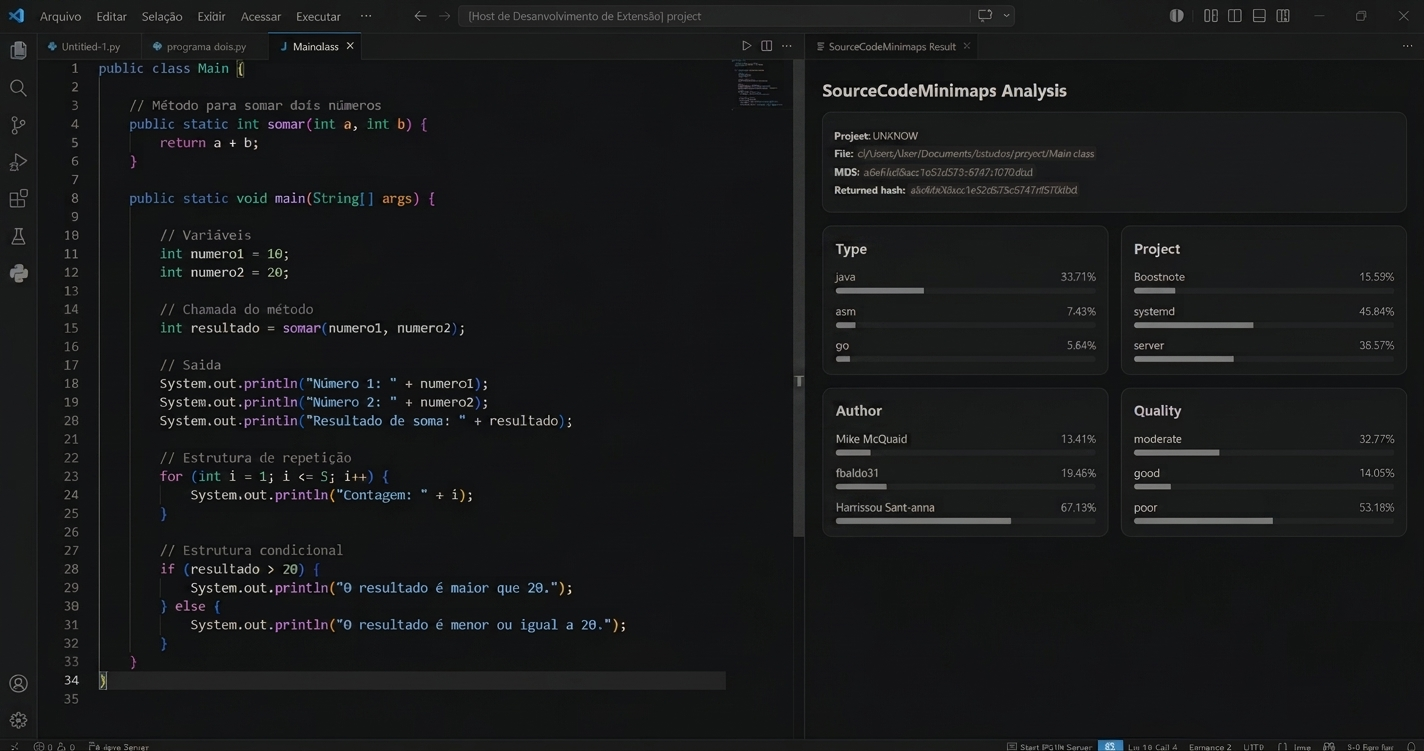
\includegraphics[width=0.92\textwidth]{figuras/vscode-plugin.png}
    \fautor
\end{figure}

The WebView approach is useful for richer visual feedback. It can present cards,
confidence bars, minimap images, and future XAI overlays. This makes it suitable
for exploratory workflows in which a developer wants to inspect files, folders,
or project-level patterns.

\section{IntelliJ IDEA Plugin}

The IntelliJ IDEA plugin follows a lighter interaction model. It captures the
active source artifact, generates the minimap, sends it to the backend, and
displays a Markdown-based report in a split-screen editor. This approach
integrates naturally with the IDE because the result appears as a document beside
the source file.

Figure~\ref{fig:intellij-plugin} shows the IntelliJ IDEA plugin interface.

\begin{figure}[ht]
    \centering
    \caption{IntelliJ IDEA plugin displaying a Markdown report generated from minimap analysis.}
    \label{fig:intellij-plugin}
    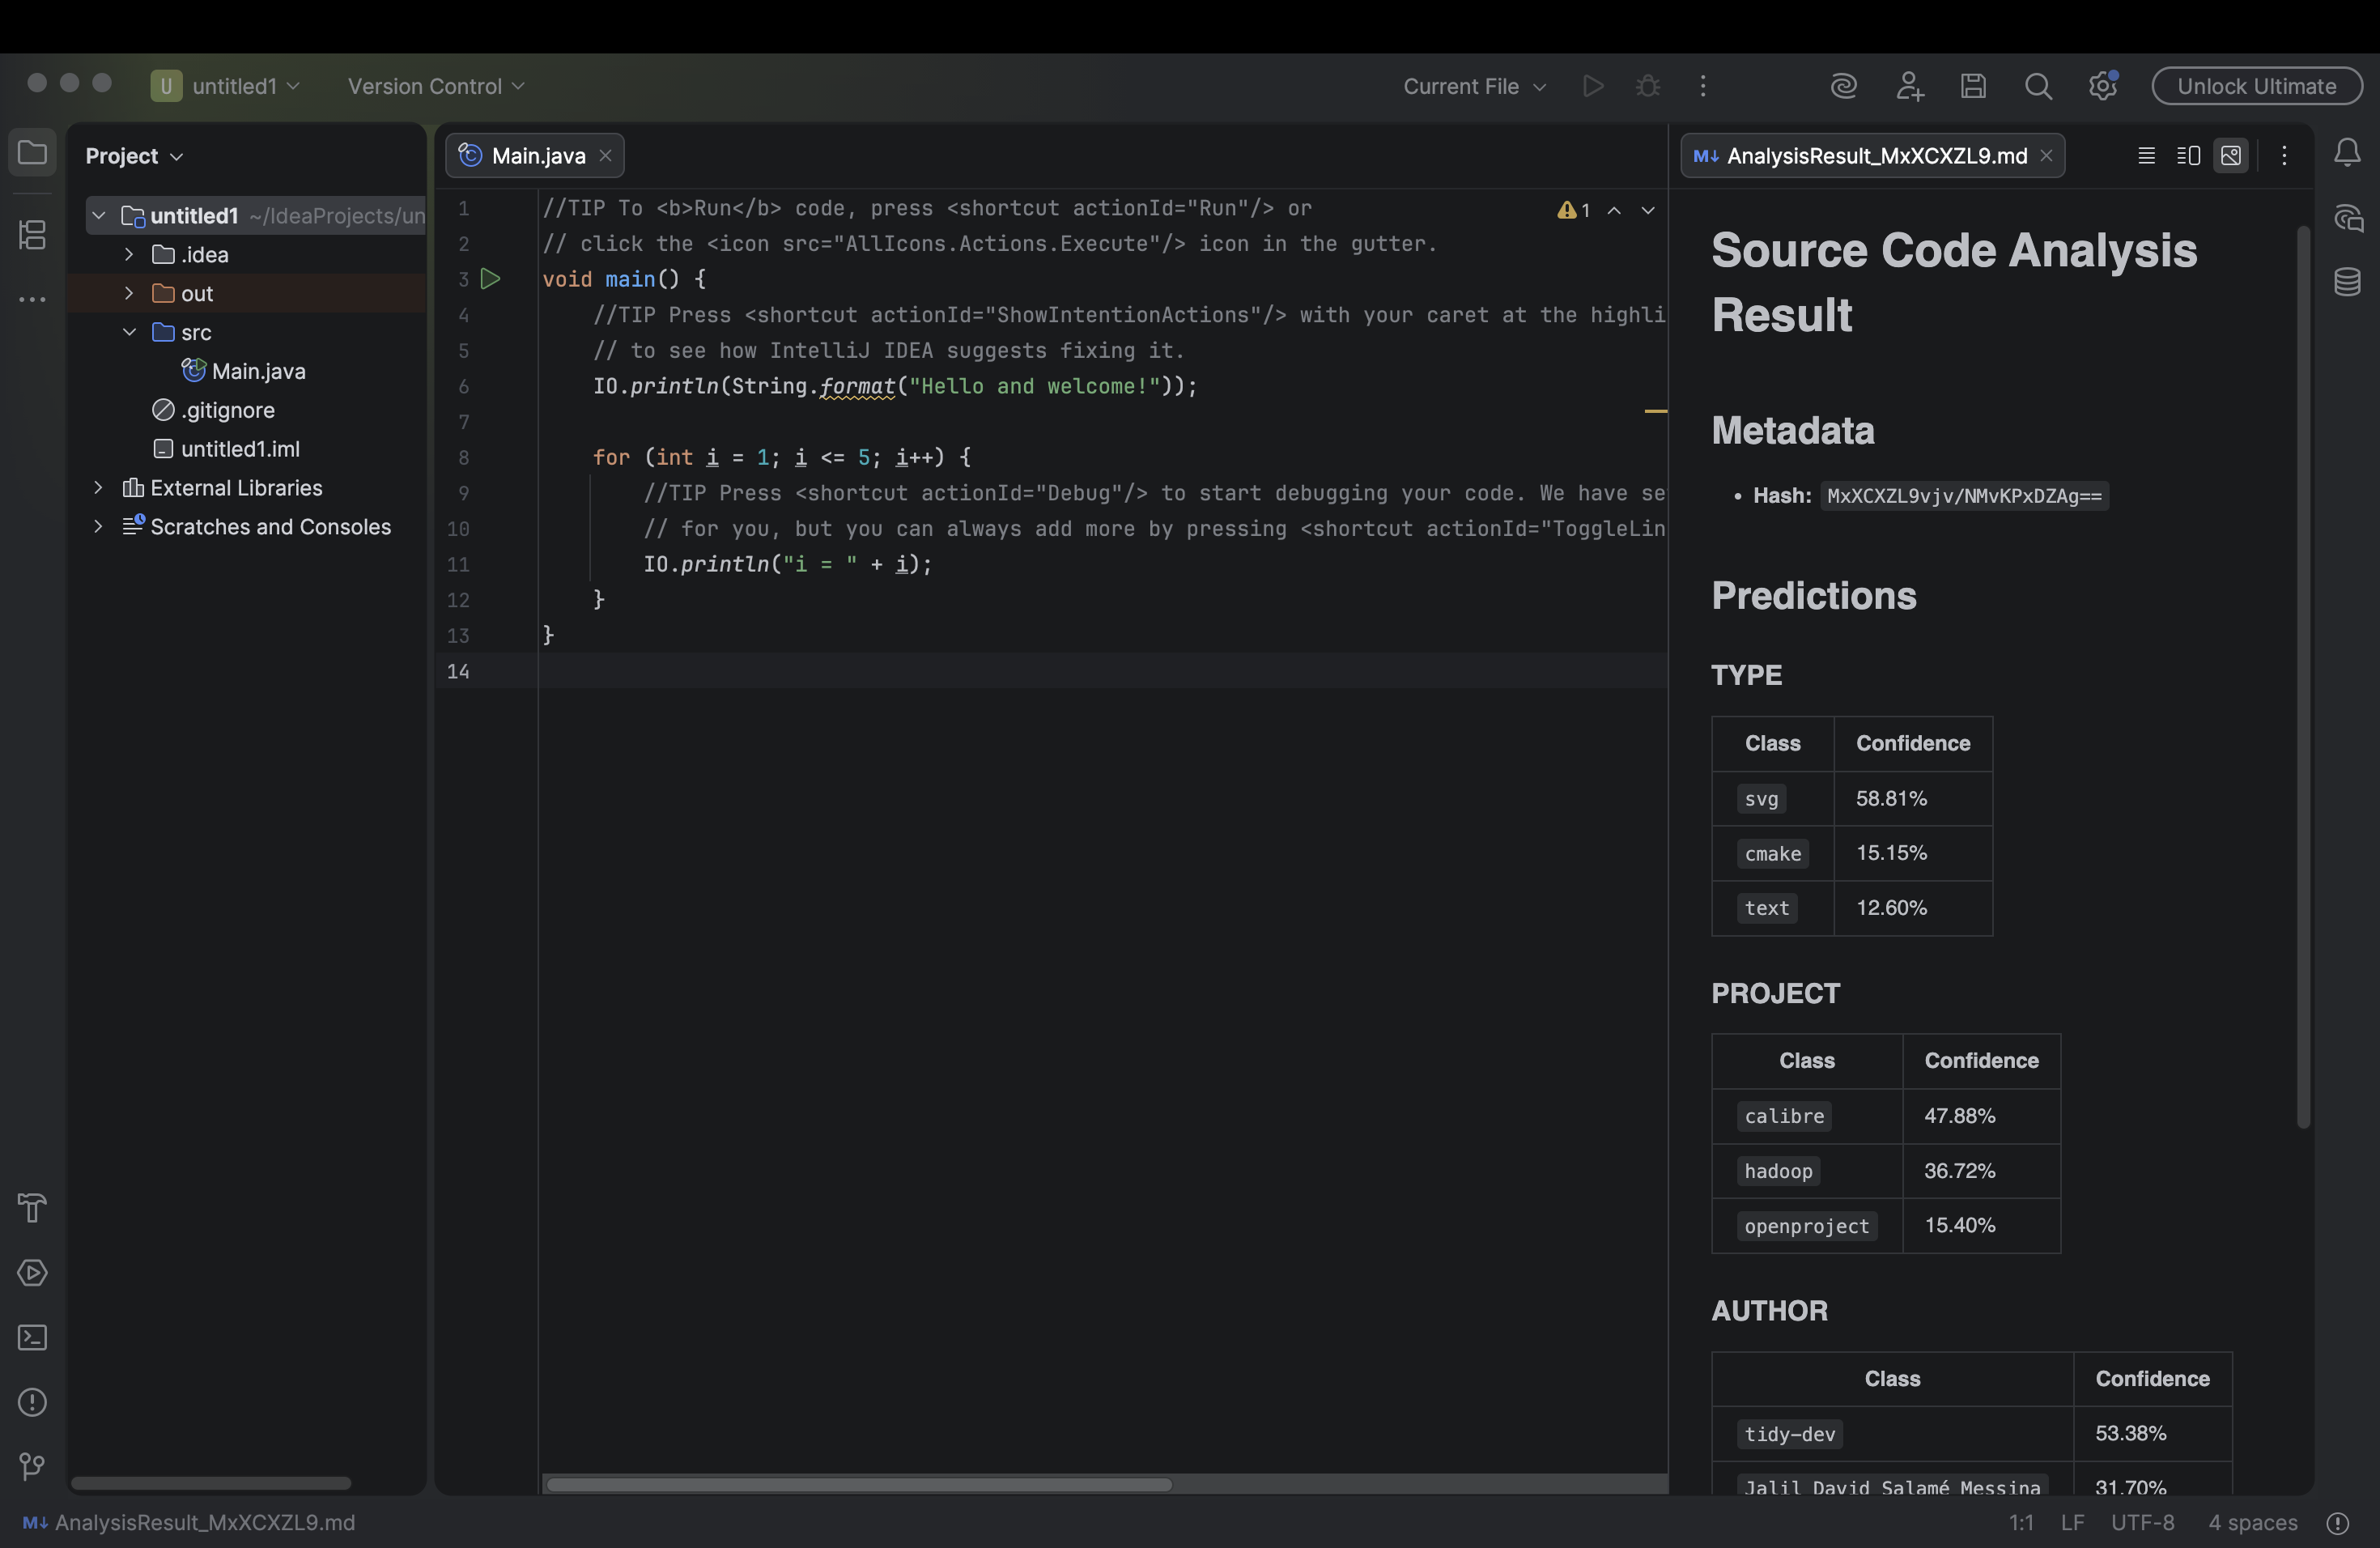
\includegraphics[width=0.92\textwidth]{figuras/intellij-plugin.png}
    \fautor
\end{figure}

The Markdown approach is less visually elaborate than the WebView interface, but
it is simple, robust, and aligned with quick inspection. It also produces a
textual artifact that can be saved, shared, or attached to later analysis.

\section{Shared Client--Server Contract}

Both IDE clients follow the same conceptual contract. Table~\ref{tab:tool-contract}
summarizes the main request and response elements.

\begin{table}[ht]
\centering
\caption{Shared client--server contract in MinimapSignatures.}
\label{tab:tool-contract}
\begin{tabular}{p{0.22\textwidth}p{0.58\textwidth}}
\toprule
\textbf{Element} & \textbf{Description} \\
\midrule
Project identifier & Optional or inferred identifier for the current workspace. \\
Artifact hash & Stable hash used to identify the analyzed file without sending its path in clear text. \\
Minimap image & Base64-encoded PNG generated locally by the IDE client. \\
Model group & Prediction target such as Type, Project, or Author. \\
Predicted label & Most likely class returned by the backend. \\
Confidence score & Numeric score associated with the prediction. \\
Additional metadata & Optional fields for model version, preprocessing mode, or explanation data. \\
\bottomrule
\end{tabular}
\fautor
\end{table}

The shared contract confirms that minimap-based analysis is not tied to a single
IDE. Additional clients can be implemented by generating the same minimap format
and sending the same request structure.

\section{Functional Validation}

The current evaluation of MinimapSignatures is functional and
integration-oriented. It verifies whether the complete workflow can be executed
successfully. Table~\ref{tab:functional-validation} summarizes the validation
status.

\begin{table}[ht]
\centering
\caption{Functional validation of MinimapSignatures.}
\label{tab:functional-validation}
\begin{tabular}{p{0.58\textwidth}p{0.20\textwidth}}
\toprule
\textbf{Component or feature} & \textbf{Status} \\
\midrule
Backend receives base64 minimap payloads & Validated \\
Backend preprocesses images for inference & Validated \\
Backend invokes trained models & Validated \\
Backend returns structured prediction groups & Validated \\
Visual Studio Code extension generates and submits minimaps & Validated \\
Visual Studio Code extension displays WebView results & Validated \\
IntelliJ IDEA plugin generates and submits minimaps & Validated \\
IntelliJ IDEA plugin displays Markdown results & Validated \\
Shared client--server contract works across IDEs & Validated \\
Multi-file and project-level analysis & Planned \\
Project-specific model update & Planned \\
Developer usability evaluation & Planned \\
\bottomrule
\end{tabular}
\fautor
\end{table}

This validation does not yet demonstrate that the tool improves productivity,
reduces comprehension effort, or increases trust. Those claims require a
different evaluation design, such as observational studies, controlled tasks,
interviews, or field deployments. At this stage, the contribution is that the
research pipeline can be executed from real IDEs.

\section{Usage Scenarios}

MinimapSignatures can support several usage scenarios. The current prototype
implements only part of them, but they guide future development and evaluation.

\subsection{Single-File Inspection}

In the simplest scenario, a developer opens a file and triggers minimap analysis.
The tool returns the predicted Type, optional Project or style-related
predictions, confidence scores, and later an explanation overlay. This scenario
is useful when a developer inspects an unfamiliar file and wants a quick
classification or when a reviewer wants to compare a file against expected
roles.

\subsection{Code Review Support}

During code review, a pull request may introduce files that visually differ from
the existing project conventions. A minimap-based tool could flag unusual
artifacts for additional inspection. The output should be framed carefully: the
tool should not say that a file is wrong, but that it is visually unusual
relative to a learned distribution. This makes the tool a prioritization aid.

\subsection{Onboarding and Repository Exploration}

A new developer entering a project often needs to understand file roles and
project organization. A project-level version of MinimapSignatures could render
minimaps for selected folders, group similar artifacts, and summarize dominant
file patterns. Such a view would complement textual navigation and dependency
analysis.

\subsection{Project-Specific Model Adaptation}

Organizations may have conventions that differ from open-source datasets. A
future version of the tool could allow teams to generate a private minimap
catalog and train or fine-tune project-specific models. This would make the
analysis more relevant to local architecture, naming patterns, and quality
expectations, while still avoiding transmission of raw source code.

\section{Artifact Availability and Repositories}

The public code organization for the project is
\url{https://github.com/minimap-project}. At the time this document was prepared,
the organization included repositories for the training infrastructure,
shared assets, backend service, IntelliJ IDEA plugin, and Visual Studio Code
extension. The artifact structure supports separation of concerns:

\begin{itemize}
    \item \texttt{minimap-signatures-trainer}: training and model-related code;
    \item \texttt{assets}: shared visual and documentation assets;
    \item \texttt{back-end}: Python inference backend;
    \item \texttt{intellij-plugin}: IntelliJ IDEA client;
    \item \texttt{vscode-plugin}: Visual Studio Code client.
\end{itemize}

This organization is useful for research reproducibility because it avoids
mixing IDE-specific code with training scripts and backend inference logic. It
also allows each component to evolve independently. For example, a new model can
be added to the backend without changing the extension packaging, while a new
IDE client can reuse the same backend contract.

\section{Planned Extensions}

The next versions of MinimapSignatures should support four extensions.

First, the tool should move from single-file analysis to multi-file and
project-level analysis. This would allow developers to inspect a folder, module,
or entire repository and receive summaries of visual signatures, unusual files,
or clusters of similar artifacts.

Second, the backend should support explanation maps. Integrated Gradients or
other attribution methods can be computed server-side and returned to the IDE so
that developers can see which regions influenced predictions. This would make
the tool more transparent than a label-only classifier.

Third, the tool should support project-specific model customization. A team may
want to train or adapt a model using its own conventions, especially for
architectural roles or quality indicators. The minimap catalog and backend
architecture can support this direction.

Fourth, the tool should include quality-related targets. Instead of predicting
only Type, Project, or Author, future models may identify code-smell likelihood,
architectural deviation, generated-file anomalies, suspicious templates, or
files that deserve priority in code review.

These extensions will move the tool from proof of integration toward a research
platform for developer-facing visual source code analysis.
